\subsection{2021年5月7日}
\paragraph{\href{https://www.51voa.com/VOA_Special_English/more-support-easing-vaccine-patent-rules-but-problems-remain-more-support-easing-vaccine-patent-rules-but-problems-remain-86814.html}{原文}}

\begin{figure}[H]
\centering
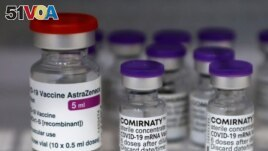
\includegraphics[scale=0.7]{007_voa_20210507.jpg}
\caption{Vials of the AstraZeneca and Pfizer-BioNTech Comirnaty coronavirus disease (COVID-19) vaccines are pictured in a General practitioners practice in Berlin, Germany, April 10, 2021.}
\end{figure}

By Susan Shand
06 May 2021
France joined the United States on Thursday in support of easing patent protections on COVID-19 vaccines. The action could help poorer countries get more shots and quicken the end of the pandemic.
On Wednesday, the U.S. government changed its own position and supported removing the protections. It brought cheers from health activists and complaints from drug companies.
During a visit to a vaccine center on Thursday, French President Emmanuel Macron added, "I completely favor this opening up of the intellectual property."
Despite his support for removing protections, Macron also said it would not solve the problem of getting more vaccines to more people around the world. He noted that places like Africa were not equipped to make COVID-19 vaccines. He said vaccine donation should be most important.
While the backing from two countries with big drug making companies is important, many problems remain to be solved.
The idea of removing patent protections was first floated by India and South Africa in October.
Some 80 countries, mostly developing nations, have supported the Indian and South African idea, an official who was not permitted to give his name said.
However, if one country in the World Trade Organization (WTO) votes against the plan, it will block efforts to make the change.
Australian Prime Minister Scott Morrison called the U.S. announcement "great news," but did not answer a question about whether his country would make the same decision. South Korean officials said they were also watching the Biden announcement, but did not say they would do the same.
Russian President Vladimir Putin said his country would support it.
The drug industry says that a faster answer to the lack of vaccines in some parts of the world would be for rich countries to start sharing their vaccine supply with poorer countries.
The industry argues that production of coronavirus vaccines is difficult and cannot be increased by easing intellectual property protections. Instead, it says that reducing problems in supply chains as well as the lack of vaccine ingredients are the most important problems right now.
"A waiver is the simple but the wrong answer to what is a complex problem," said the International Federation of Pharmaceutical Manufacturers and Associations. The organization added that the idea "will not increase production nor provide practical solutions" to the health crisis.
Intellectual property expert Shyam Balganesh is a professor at Columbia Law School. He said a WTO waiver could help but it would only go so far because of other problems in the manufacturing and shipping of vaccines.
I'm Jonathan Evans.
The Associated Press reported this story. Susan Shand adapted it for Learning English. Hai Do was the editor.

\begin{messagebox}
Words in This Story
patent – n. an official document that gives a person or company the right to be the only one that makes or sells a product for a certain period of time
summit – n. a meeting or series of meetings between the leaders of two or more governments
waiver – n. an official document indicating that someone has given up or waived a right or requirement
complex – adj. not easy to understand or explain : not simple
\end{messagebox}

France joined the United States on Thursday in support of easing patent protections on COVID-19 vaccines. The action could help poorer countries get more shots and quicken the end of the pandemic.
法国周四加入美国支持放宽对新冠肺炎疫苗的专利保护。此举可以帮助贫困国家获得更多疫苗,并加快大流行的终结。
On Wednesday, the U.S. government changed its own position and supported removing the protections. It brought cheers from health activists and complaints from drug companies.
周三,美国政府改变了自身立场,支持豁免这些专利保护。这引起了卫生活动人士的欢呼与制药公司的抱怨。

During a visit to a vaccine center on Thursday, French President Emmanuel Macron added, "I completely favor this opening up of the intellectual property."
法国总统马克龙周四在视察一家疫苗中心时还表示:“我完全赞成开放这种知识产权。”

Despite his support for removing protections, Macron also said it would not solve the problem of getting more vaccines to more people around the world. He noted that places like Africa were not equipped to make COVID-19 vaccines. He said vaccine donation should be most important.
尽管马克龙支持豁免专利保护,但他也表示,这无法解决向世界上更多人提供更多疫苗的问题。他指出,像非洲这样的地区不具备生产新冠肺炎疫苗的条件。他说捐赠疫苗应该是最重要的。

While the backing from two countries with big drug making companies is important, many problems remain to be solved.
这两个拥有大型制药公司的国家的支持固然重要,但是仍有问题有待解决。

The idea of removing patent protections was first floated by India and South Africa in October.
印度和南非在去年10月份首先提出了豁免专利保护的想法。

Some 80 countries, mostly developing nations, have supported the Indian and South African idea, an official who was not permitted to give his name said.
一位不愿意透露姓名的官员表示,大约有80个国家支持印度和南非的想法,其中大多数是发展中国家。

However, if one country in the World Trade Organization (WTO) votes against the plan, it will block efforts to make the change.
然而,如果世贸组织的某个国家投票反对这项计划,它将阻碍这种改革的努力。

Australian Prime Minister Scott Morrison called the U.S. announcement "great news," but did not answer a question about whether his country would make the same decision. South Korean officials said they were also watching the Biden announcement, but did not say they would do the same.
澳大利亚总理莫里森称美国的声明是“重大新闻,”但是并未回答有关澳大利亚是否会做出同样决定的提问。韩国官员表示,他们也正在观看拜登的声明,但是并未表态他们也会这样做。

Russian President Vladimir Putin said his country would support it.
俄罗斯总统普京称俄罗斯支持这样做。

The drug industry says that a faster answer to the lack of vaccines in some parts of the world would be for rich countries to start sharing their vaccine supply with poorer countries.
制药行业表示,对于世界部分地区的疫苗短缺问题,较快的解决途径是发达国家向贫困国家分享疫苗供应。

The industry argues that production of coronavirus vaccines is difficult and cannot be increased by easing intellectual property protections. Instead, it says that reducing problems in supply chains as well as the lack of vaccine ingredients are the most important problems right now.
业界认为,新冠病毒疫苗的生产很难,无法通过放宽知识产权保护来提高生产。相反,减少供应链的问题以及疫苗原料的短缺是目前最重要的问题。

"A waiver is the simple but the wrong answer to what is a complex problem," said the International Federation of Pharmaceutical Manufacturers and Associations. The organization added that the idea "will not increase production nor provide practical solutions" to the health crisis.
国际制药商联合会表示:“放弃知识产权很简单,但却是解决这个复杂问题的错误答案。”该组织还表示,这种想法无法提高产量,也无法提供对这次健康危机的实用解决方案。

Intellectual property expert Shyam Balganesh is a professor at Columbia Law School. He said a WTO waiver could help but it would only go so far because of other problems in the manufacturing and shipping of vaccines.
知识产权专家Shyam Balganesh是哥伦比亚大学法学院的教授。他说,世卫组织的豁免可能会有帮助,但是由于疫苗生产和运输中的其它问题,它的作用不过如此。
